\documentclass[tikz,border=10pt]{standalone}
\usetikzlibrary{calc}
\begin{document}
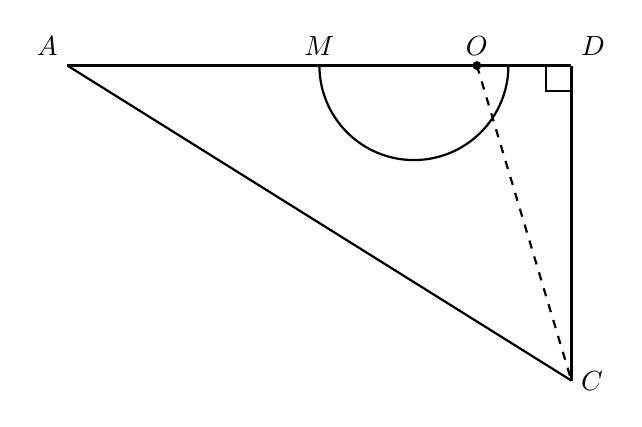
\begin{tikzpicture}[scale=0.8]
\coordinate (A) at (0,0);
\coordinate (M) at (4,0);
\coordinate (O) at (6.5,0);
\coordinate (D) at (8,0);
\coordinate (C) at (8,-5);

\draw[thick] (A) -- (D);
\draw[thick] (D) -- (C);
\draw[thick] (A) -- (C);
\draw[thick] (M) arc[start angle=180, end angle=360, radius=1.5];
\draw[dashed, thick] (O) -- (C);

% right-angle mark at D
\draw[thick] (7.6,0) -- (7.6,-0.4) -- (8,-0.4);

\fill (O) circle (2pt);

\node[above left] at (A) {$A$};
\node[above] at (M) {$M$};
\node[above] at (O) {$O$};
\node[above right] at (D) {$D$};
\node[right] at (C) {$C$};
\end{tikzpicture}
\end{document}
